% Options for packages loaded elsewhere
\PassOptionsToPackage{unicode}{hyperref}
\PassOptionsToPackage{hyphens}{url}
%
\documentclass[
  letterpaper,
]{book}

\usepackage{amsmath,amssymb}
\usepackage{iftex}
\ifPDFTeX
  \usepackage[T1]{fontenc}
  \usepackage[utf8]{inputenc}
  \usepackage{textcomp} % provide euro and other symbols
\else % if luatex or xetex
  \usepackage{unicode-math}
  \defaultfontfeatures{Scale=MatchLowercase}
  \defaultfontfeatures[\rmfamily]{Ligatures=TeX,Scale=1}
\fi
\usepackage{lmodern}
\ifPDFTeX\else  
    % xetex/luatex font selection
\fi
% Use upquote if available, for straight quotes in verbatim environments
\IfFileExists{upquote.sty}{\usepackage{upquote}}{}
\IfFileExists{microtype.sty}{% use microtype if available
  \usepackage[]{microtype}
  \UseMicrotypeSet[protrusion]{basicmath} % disable protrusion for tt fonts
}{}
\makeatletter
\@ifundefined{KOMAClassName}{% if non-KOMA class
  \IfFileExists{parskip.sty}{%
    \usepackage{parskip}
  }{% else
    \setlength{\parindent}{0pt}
    \setlength{\parskip}{6pt plus 2pt minus 1pt}}
}{% if KOMA class
  \KOMAoptions{parskip=half}}
\makeatother
\usepackage{xcolor}
\setlength{\emergencystretch}{3em} % prevent overfull lines
\setcounter{secnumdepth}{5}
% Make \paragraph and \subparagraph free-standing
\makeatletter
\ifx\paragraph\undefined\else
  \let\oldparagraph\paragraph
  \renewcommand{\paragraph}{
    \@ifstar
      \xxxParagraphStar
      \xxxParagraphNoStar
  }
  \newcommand{\xxxParagraphStar}[1]{\oldparagraph*{#1}\mbox{}}
  \newcommand{\xxxParagraphNoStar}[1]{\oldparagraph{#1}\mbox{}}
\fi
\ifx\subparagraph\undefined\else
  \let\oldsubparagraph\subparagraph
  \renewcommand{\subparagraph}{
    \@ifstar
      \xxxSubParagraphStar
      \xxxSubParagraphNoStar
  }
  \newcommand{\xxxSubParagraphStar}[1]{\oldsubparagraph*{#1}\mbox{}}
  \newcommand{\xxxSubParagraphNoStar}[1]{\oldsubparagraph{#1}\mbox{}}
\fi
\makeatother

\usepackage{color}
\usepackage{fancyvrb}
\newcommand{\VerbBar}{|}
\newcommand{\VERB}{\Verb[commandchars=\\\{\}]}
\DefineVerbatimEnvironment{Highlighting}{Verbatim}{commandchars=\\\{\}}
% Add ',fontsize=\small' for more characters per line
\usepackage{framed}
\definecolor{shadecolor}{RGB}{241,243,245}
\newenvironment{Shaded}{\begin{snugshade}}{\end{snugshade}}
\newcommand{\AlertTok}[1]{\textcolor[rgb]{0.68,0.00,0.00}{#1}}
\newcommand{\AnnotationTok}[1]{\textcolor[rgb]{0.37,0.37,0.37}{#1}}
\newcommand{\AttributeTok}[1]{\textcolor[rgb]{0.40,0.45,0.13}{#1}}
\newcommand{\BaseNTok}[1]{\textcolor[rgb]{0.68,0.00,0.00}{#1}}
\newcommand{\BuiltInTok}[1]{\textcolor[rgb]{0.00,0.23,0.31}{#1}}
\newcommand{\CharTok}[1]{\textcolor[rgb]{0.13,0.47,0.30}{#1}}
\newcommand{\CommentTok}[1]{\textcolor[rgb]{0.37,0.37,0.37}{#1}}
\newcommand{\CommentVarTok}[1]{\textcolor[rgb]{0.37,0.37,0.37}{\textit{#1}}}
\newcommand{\ConstantTok}[1]{\textcolor[rgb]{0.56,0.35,0.01}{#1}}
\newcommand{\ControlFlowTok}[1]{\textcolor[rgb]{0.00,0.23,0.31}{\textbf{#1}}}
\newcommand{\DataTypeTok}[1]{\textcolor[rgb]{0.68,0.00,0.00}{#1}}
\newcommand{\DecValTok}[1]{\textcolor[rgb]{0.68,0.00,0.00}{#1}}
\newcommand{\DocumentationTok}[1]{\textcolor[rgb]{0.37,0.37,0.37}{\textit{#1}}}
\newcommand{\ErrorTok}[1]{\textcolor[rgb]{0.68,0.00,0.00}{#1}}
\newcommand{\ExtensionTok}[1]{\textcolor[rgb]{0.00,0.23,0.31}{#1}}
\newcommand{\FloatTok}[1]{\textcolor[rgb]{0.68,0.00,0.00}{#1}}
\newcommand{\FunctionTok}[1]{\textcolor[rgb]{0.28,0.35,0.67}{#1}}
\newcommand{\ImportTok}[1]{\textcolor[rgb]{0.00,0.46,0.62}{#1}}
\newcommand{\InformationTok}[1]{\textcolor[rgb]{0.37,0.37,0.37}{#1}}
\newcommand{\KeywordTok}[1]{\textcolor[rgb]{0.00,0.23,0.31}{\textbf{#1}}}
\newcommand{\NormalTok}[1]{\textcolor[rgb]{0.00,0.23,0.31}{#1}}
\newcommand{\OperatorTok}[1]{\textcolor[rgb]{0.37,0.37,0.37}{#1}}
\newcommand{\OtherTok}[1]{\textcolor[rgb]{0.00,0.23,0.31}{#1}}
\newcommand{\PreprocessorTok}[1]{\textcolor[rgb]{0.68,0.00,0.00}{#1}}
\newcommand{\RegionMarkerTok}[1]{\textcolor[rgb]{0.00,0.23,0.31}{#1}}
\newcommand{\SpecialCharTok}[1]{\textcolor[rgb]{0.37,0.37,0.37}{#1}}
\newcommand{\SpecialStringTok}[1]{\textcolor[rgb]{0.13,0.47,0.30}{#1}}
\newcommand{\StringTok}[1]{\textcolor[rgb]{0.13,0.47,0.30}{#1}}
\newcommand{\VariableTok}[1]{\textcolor[rgb]{0.07,0.07,0.07}{#1}}
\newcommand{\VerbatimStringTok}[1]{\textcolor[rgb]{0.13,0.47,0.30}{#1}}
\newcommand{\WarningTok}[1]{\textcolor[rgb]{0.37,0.37,0.37}{\textit{#1}}}

\providecommand{\tightlist}{%
  \setlength{\itemsep}{0pt}\setlength{\parskip}{0pt}}\usepackage{longtable,booktabs,array}
\usepackage{calc} % for calculating minipage widths
% Correct order of tables after \paragraph or \subparagraph
\usepackage{etoolbox}
\makeatletter
\patchcmd\longtable{\par}{\if@noskipsec\mbox{}\fi\par}{}{}
\makeatother
% Allow footnotes in longtable head/foot
\IfFileExists{footnotehyper.sty}{\usepackage{footnotehyper}}{\usepackage{footnote}}
\makesavenoteenv{longtable}
\usepackage{graphicx}
\makeatletter
\newsavebox\pandoc@box
\newcommand*\pandocbounded[1]{% scales image to fit in text height/width
  \sbox\pandoc@box{#1}%
  \Gscale@div\@tempa{\textheight}{\dimexpr\ht\pandoc@box+\dp\pandoc@box\relax}%
  \Gscale@div\@tempb{\linewidth}{\wd\pandoc@box}%
  \ifdim\@tempb\p@<\@tempa\p@\let\@tempa\@tempb\fi% select the smaller of both
  \ifdim\@tempa\p@<\p@\scalebox{\@tempa}{\usebox\pandoc@box}%
  \else\usebox{\pandoc@box}%
  \fi%
}
% Set default figure placement to htbp
\def\fps@figure{htbp}
\makeatother
% definitions for citeproc citations
\NewDocumentCommand\citeproctext{}{}
\NewDocumentCommand\citeproc{mm}{%
  \begingroup\def\citeproctext{#2}\cite{#1}\endgroup}
\makeatletter
 % allow citations to break across lines
 \let\@cite@ofmt\@firstofone
 % avoid brackets around text for \cite:
 \def\@biblabel#1{}
 \def\@cite#1#2{{#1\if@tempswa , #2\fi}}
\makeatother
\newlength{\cslhangindent}
\setlength{\cslhangindent}{1.5em}
\newlength{\csllabelwidth}
\setlength{\csllabelwidth}{3em}
\newenvironment{CSLReferences}[2] % #1 hanging-indent, #2 entry-spacing
 {\begin{list}{}{%
  \setlength{\itemindent}{0pt}
  \setlength{\leftmargin}{0pt}
  \setlength{\parsep}{0pt}
  % turn on hanging indent if param 1 is 1
  \ifodd #1
   \setlength{\leftmargin}{\cslhangindent}
   \setlength{\itemindent}{-1\cslhangindent}
  \fi
  % set entry spacing
  \setlength{\itemsep}{#2\baselineskip}}}
 {\end{list}}
\usepackage{calc}
\newcommand{\CSLBlock}[1]{\hfill\break\parbox[t]{\linewidth}{\strut\ignorespaces#1\strut}}
\newcommand{\CSLLeftMargin}[1]{\parbox[t]{\csllabelwidth}{\strut#1\strut}}
\newcommand{\CSLRightInline}[1]{\parbox[t]{\linewidth - \csllabelwidth}{\strut#1\strut}}
\newcommand{\CSLIndent}[1]{\hspace{\cslhangindent}#1}

\usepackage{booktabs}
\usepackage{longtable}
\usepackage{array}
\usepackage{multirow}
\usepackage{wrapfig}
\usepackage{float}
\usepackage{colortbl}
\usepackage{pdflscape}
\usepackage{tabu}
\usepackage{threeparttable}
\usepackage{threeparttablex}
\usepackage[normalem]{ulem}
\usepackage{makecell}
\usepackage{xcolor}
\makeatletter
\@ifpackageloaded{tcolorbox}{}{\usepackage[skins,breakable]{tcolorbox}}
\@ifpackageloaded{fontawesome5}{}{\usepackage{fontawesome5}}
\definecolor{quarto-callout-color}{HTML}{909090}
\definecolor{quarto-callout-note-color}{HTML}{0758E5}
\definecolor{quarto-callout-important-color}{HTML}{CC1914}
\definecolor{quarto-callout-warning-color}{HTML}{EB9113}
\definecolor{quarto-callout-tip-color}{HTML}{00A047}
\definecolor{quarto-callout-caution-color}{HTML}{FC5300}
\definecolor{quarto-callout-color-frame}{HTML}{acacac}
\definecolor{quarto-callout-note-color-frame}{HTML}{4582ec}
\definecolor{quarto-callout-important-color-frame}{HTML}{d9534f}
\definecolor{quarto-callout-warning-color-frame}{HTML}{f0ad4e}
\definecolor{quarto-callout-tip-color-frame}{HTML}{02b875}
\definecolor{quarto-callout-caution-color-frame}{HTML}{fd7e14}
\makeatother
\makeatletter
\@ifpackageloaded{bookmark}{}{\usepackage{bookmark}}
\makeatother
\makeatletter
\@ifpackageloaded{caption}{}{\usepackage{caption}}
\AtBeginDocument{%
\ifdefined\contentsname
  \renewcommand*\contentsname{Table of contents}
\else
  \newcommand\contentsname{Table of contents}
\fi
\ifdefined\listfigurename
  \renewcommand*\listfigurename{List of Figures}
\else
  \newcommand\listfigurename{List of Figures}
\fi
\ifdefined\listtablename
  \renewcommand*\listtablename{List of Tables}
\else
  \newcommand\listtablename{List of Tables}
\fi
\ifdefined\figurename
  \renewcommand*\figurename{Figure}
\else
  \newcommand\figurename{Figure}
\fi
\ifdefined\tablename
  \renewcommand*\tablename{Table}
\else
  \newcommand\tablename{Table}
\fi
}
\@ifpackageloaded{float}{}{\usepackage{float}}
\floatstyle{ruled}
\@ifundefined{c@chapter}{\newfloat{codelisting}{h}{lop}}{\newfloat{codelisting}{h}{lop}[chapter]}
\floatname{codelisting}{Listing}
\newcommand*\listoflistings{\listof{codelisting}{List of Listings}}
\makeatother
\makeatletter
\makeatother
\makeatletter
\@ifpackageloaded{caption}{}{\usepackage{caption}}
\@ifpackageloaded{subcaption}{}{\usepackage{subcaption}}
\makeatother

\usepackage{bookmark}

\IfFileExists{xurl.sty}{\usepackage{xurl}}{} % add URL line breaks if available
\urlstyle{same} % disable monospaced font for URLs
\hypersetup{
  pdftitle={Manutenção e Confiabilidade: Aplicação em R},
  pdfauthor={Rafael da Silva Fernandes},
  hidelinks,
  pdfcreator={LaTeX via pandoc}}


\title{Manutenção e Confiabilidade: Aplicação em R}
\usepackage{etoolbox}
\makeatletter
\providecommand{\subtitle}[1]{% add subtitle to \maketitle
  \apptocmd{\@title}{\par {\large #1 \par}}{}{}
}
\makeatother
\subtitle{Aplicações em R}
\author{Rafael da Silva Fernandes}
\date{2025-11-26}

\begin{document}
\frontmatter
\maketitle

\renewcommand*\contentsname{Table of contents}
{
\setcounter{tocdepth}{2}
\tableofcontents
}

\mainmatter
\chapter{Manutenção e Confiabilidade: Aplicação em
R}\label{manutenuxe7uxe3o-e-confiabilidade-aplicauxe7uxe3o-em-r}

\chapter*{Bem-vindo}\label{bem-vindo}
\addcontentsline{toc}{chapter}{Bem-vindo}

\markboth{Bem-vindo}{Bem-vindo}

Bem-vindo ao livro \textbf{``Confiabilidade e Manutenção: Princípios e
Prática''}!

\begin{tcolorbox}[enhanced jigsaw, opacityback=0, leftrule=.75mm, colback=white, bottomrule=.15mm, arc=.35mm, toprule=.15mm, rightrule=.15mm, left=2mm, colframe=quarto-callout-note-color-frame, breakable]
\begin{minipage}[t]{5.5mm}
\textcolor{quarto-callout-note-color}{\faInfo}
\end{minipage}%
\begin{minipage}[t]{\textwidth - 5.5mm}

\vspace{-3mm}\textbf{Sobre este Livro}\vspace{3mm}

Este livro fornece uma introdução \textbf{prática e aplicada} aos
conceitos de confiabilidade, análise de dados de falha e modelagem de
vida útil, com ênfase no uso da linguagem \textbf{R} como ferramenta
principal.

\end{minipage}%
\end{tcolorbox}

\section{📚 O que você vai aprender}\label{o-que-vocuxea-vai-aprender}

\begin{itemize}
\tightlist
\item
  \textbf{Fundamentos de confiabilidade} --- Conceitos, métricas e
  distribuições de vida útil
\item
  \textbf{Análise de dados de falha} --- Técnicas estatísticas para
  dados censurados
\item
  \textbf{Modelagem Weibull} --- Aplicação prática da distribuição mais
  usada em engenharia
\item
  \textbf{Análise de sobrevivência} --- Modelos paramétricos e
  semiparamétricos
\item
  \textbf{Estratégias de manutenção} --- Otimização de políticas
  preventivas e preditivas
\item
  \textbf{Machine learning} --- Predição de falhas com dados de sensores
\item
  \textbf{Simulação Monte Carlo} --- Avaliação de políticas sob
  incerteza
\item
  \textbf{Boas práticas} --- Governança de dados e reprodutibilidade
\end{itemize}

\section{🎯 Para quem é este livro}\label{para-quem-uxe9-este-livro}

\begin{itemize}
\tightlist
\item
  \textbf{Engenheiros de confiabilidade e manutenção}
\item
  \textbf{Analistas de dados} em contextos industriais
\item
  \textbf{Estudantes e pesquisadores} em engenharia e estatística
\item
  \textbf{Gestores técnicos} que tomam decisões baseadas em dados
\end{itemize}

\section{🚀 Como usar este livro}\label{como-usar-este-livro}

\begin{enumerate}
\def\labelenumi{\arabic{enumi}.}
\tightlist
\item
  \textbf{Leia sequencialmente} --- Os capítulos são progressivos
\item
  \textbf{Execute os exemplos} --- Todos os códigos R são reproduzíveis
\item
  \textbf{Faça os exercícios} --- Pratique para consolidar o aprendizado
\item
  \textbf{Use como referência} --- Consulte os apêndices quando
  necessário
\end{enumerate}

\section{📖 Estrutura}\label{estrutura}

O livro está organizado em \textbf{quatro partes principais}:

\begin{itemize}
\tightlist
\item
  \textbf{Parte I:} Contexto de Mineração
\item
  \textbf{Parte II:} Fundamentos de Confiabilidade
\item
  \textbf{Parte III:} Estratégias de Manutenção
\item
  \textbf{Parte IV:} Tópicos Avançados
\end{itemize}

\section{💻 Requisitos}\label{requisitos}

\begin{itemize}
\tightlist
\item
  \textbf{R} (versão ≥ 4.0) e \textbf{RStudio} ou VS Code
\item
  \textbf{Pacotes R} principais: \texttt{tidyverse}, \texttt{survival},
  \texttt{flexsurv}, \texttt{ggplot2}
\end{itemize}

Veja instruções completas em \href{setup.qmd}{Instalação e Ambiente}.

\section{🔗 Recursos}\label{recursos}

\begin{itemize}
\tightlist
\item
  \textbf{Código:}
  \href{https://github.com/rafasfer2/QuartoBook}{GitHub}
\item
  \textbf{Dados:} Disponíveis em \texttt{resources/data/}
\item
  \textbf{Issues:}
  \href{https://github.com/rafasfer2/QuartoBook/issues}{GitHub Issues}
\end{itemize}

\begin{center}\rule{0.5\linewidth}{0.5pt}\end{center}

\begin{tcolorbox}[enhanced jigsaw, opacityback=0, leftrule=.75mm, colback=white, bottomrule=.15mm, colbacktitle=quarto-callout-tip-color!10!white, rightrule=.15mm, colframe=quarto-callout-tip-color-frame, coltitle=black, titlerule=0mm, opacitybacktitle=0.6, title=\textcolor{quarto-callout-tip-color}{\faLightbulb}\hspace{0.5em}{Pronto para começar?}, toprule=.15mm, toptitle=1mm, arc=.35mm, left=2mm, bottomtitle=1mm, breakable]

Inicie pelo \href{preface.qmd}{Prefácio} para entender melhor o contexto
e objetivos deste livro, ou vá direto para \href{requirements.qmd}{Como
Usar este Livro} para configurar seu ambiente.

\end{tcolorbox}

\begin{center}\rule{0.5\linewidth}{0.5pt}\end{center}

\textbf{Boa leitura e bons estudos!} 📊✨

\part{}

\chapter*{Prefácio}\label{prefuxe1cio}
\addcontentsline{toc}{chapter}{Prefácio}

\markboth{Prefácio}{Prefácio}

\section*{Sobre este Livro}\label{sobre-este-livro-1}
\addcontentsline{toc}{section}{Sobre este Livro}

\markright{Sobre este Livro}

A \textbf{confiabilidade} e a \textbf{manutenção} de equipamentos e
sistemas são pilares fundamentais para a operação eficiente e segura de
indústrias em todo o mundo. Com o avanço da coleta de dados, da
computação estatística e do aprendizado de máquina, a análise
quantitativa de falhas e a otimização de estratégias de manutenção
tornaram-se mais acessíveis e poderosas do que nunca.

Este livro tem como objetivo fornecer uma introdução \textbf{prática e
aplicada} aos conceitos de confiabilidade, análise de dados de falha e
modelagem de vida útil, com ênfase no uso da linguagem \textbf{R} como
ferramenta principal. Ele é direcionado a engenheiros, analistas de
dados, gestores de manutenção, estudantes e profissionais que desejam
aplicar métodos estatísticos modernos para melhorar a disponibilidade,
reduzir custos e otimizar políticas de manutenção.

\section*{Público-Alvo}\label{puxfablico-alvo}
\addcontentsline{toc}{section}{Público-Alvo}

\markright{Público-Alvo}

\begin{itemize}
\tightlist
\item
  \textbf{Engenheiros de confiabilidade e manutenção} que buscam
  ferramentas práticas para análise de dados de falha e otimização de
  políticas.
\item
  \textbf{Analistas de dados} interessados em aplicar modelos
  estatísticos e de machine learning em contextos industriais.
\item
  \textbf{Estudantes e pesquisadores} que desejam aprender técnicas de
  análise de sobrevivência e modelagem de confiabilidade com exemplos
  reais.
\item
  \textbf{Gestores técnicos} que precisam tomar decisões baseadas em
  dados para melhorar a performance de ativos.
\end{itemize}

\section*{Objetivos}\label{objetivos}
\addcontentsline{toc}{section}{Objetivos}

\markright{Objetivos}

Ao final deste livro, o leitor será capaz de:

\begin{itemize}
\tightlist
\item
  Compreender os \textbf{conceitos fundamentais} de confiabilidade,
  disponibilidade e manutenção.
\item
  Ajustar e interpretar \textbf{distribuições de vida útil} (Weibull,
  exponencial, lognormal) a dados reais.
\item
  Realizar \textbf{análise de sobrevivência} com dados censurados usando
  técnicas paramétricas e semiparamétricas.
\item
  Implementar \textbf{estratégias de manutenção preventiva e preditiva}
  com base em dados de sensores e histórico de falhas.
\item
  Utilizar \textbf{simulação Monte Carlo} para avaliar políticas de
  manutenção sob incerteza.
\item
  Aplicar boas práticas de \textbf{gestão de dados} e reprodutibilidade
  em projetos de confiabilidade.
\end{itemize}

\section*{Como Usar este Livro}\label{como-usar-este-livro-1}
\addcontentsline{toc}{section}{Como Usar este Livro}

\markright{Como Usar este Livro}

Este livro é \textbf{totalmente reproduzível}. Todos os exemplos de
código R estão embutidos nos capítulos e podem ser executados
diretamente. Recomendamos que o leitor:

\begin{enumerate}
\def\labelenumi{\arabic{enumi}.}
\tightlist
\item
  \textbf{Instale o R e o RStudio} (ou use o VS Code com extensões de R)
  seguindo as instruções no capítulo de instalação.
\item
  \textbf{Execute os exemplos} à medida que avança pelos capítulos para
  consolidar o aprendizado.
\item
  \textbf{Explore os exercícios} propostos ao final de cada capítulo
  para praticar os conceitos.
\item
  \textbf{Utilize os dados de exemplo} fornecidos na pasta
  \texttt{resources/data/} para replicar as análises.
\end{enumerate}

Os capítulos são organizados de forma \textbf{progressiva}, começando
pelos fundamentos teóricos e avançando para aplicações práticas e
estudos de caso. Você pode seguir a ordem proposta ou pular para
capítulos específicos de acordo com suas necessidades.

\section*{Ferramentas e Recursos}\label{ferramentas-e-recursos}
\addcontentsline{toc}{section}{Ferramentas e Recursos}

\markright{Ferramentas e Recursos}

Este livro foi desenvolvido com:

\begin{itemize}
\tightlist
\item
  \textbf{Quarto} --- Sistema de publicação científica e técnica que
  integra código, texto e visualizações.
\item
  \textbf{R} --- Linguagem de programação estatística open-source com
  vasto ecossistema de pacotes.
\item
  \textbf{Pacotes R principais} --- \texttt{survival},
  \texttt{flexsurv}, \texttt{WeibullR}, \texttt{reliability},
  \texttt{tidyverse}, \texttt{ggplot2}, entre outros.
\end{itemize}

Todos os materiais suplementares, incluindo dados, scripts e recursos
adicionais, estão disponíveis no diretório \texttt{resources/} do
projeto.

\section*{Convenções}\label{convenuxe7uxf5es}
\addcontentsline{toc}{section}{Convenções}

\markright{Convenções}

\begin{itemize}
\tightlist
\item
  \textbf{Código R} é apresentado em blocos destacados e pode ser
  copiado diretamente.
\item
  \textbf{Figuras e tabelas} são numeradas e referenciadas ao longo do
  texto.
\item
  \textbf{Exemplos práticos} são marcados com 💡 e \textbf{exercícios}
  com 📝.
\item
  \textbf{Dicas importantes} são destacadas com 🔔.
\end{itemize}

\section*{Agradecimentos}\label{agradecimentos}
\addcontentsline{toc}{section}{Agradecimentos}

\markright{Agradecimentos}

Este livro é fruto de anos de experiência prática em engenharia de
confiabilidade, análise de dados e ensino. Agradeço à comunidade R, aos
desenvolvedores de pacotes open-source e a todos que contribuíram com
feedback e sugestões ao longo do desenvolvimento deste material.

\begin{center}\rule{0.5\linewidth}{0.5pt}\end{center}

\textbf{Rafael da Silva Fernandes} \emph{Novembro de 2025}

\chapter*{Como Usar este Livro}\label{como-usar-este-livro-2}
\addcontentsline{toc}{chapter}{Como Usar este Livro}

\markboth{Como Usar este Livro}{Como Usar este Livro}

\section*{Convenções e
Organização}\label{convenuxe7uxf5es-e-organizauxe7uxe3o}
\addcontentsline{toc}{section}{Convenções e Organização}

\markright{Convenções e Organização}

Este livro foi desenvolvido para ser \textbf{prático, reproduzível e
didático}. Todos os exemplos de código R podem ser executados
diretamente, e os dados utilizados estão disponíveis no diretório
\texttt{resources/data/}.

\subsection*{Organização dos
Capítulos}\label{organizauxe7uxe3o-dos-capuxedtulos}
\addcontentsline{toc}{subsection}{Organização dos Capítulos}

O livro está dividido em \textbf{quatro partes principais}:

\begin{enumerate}
\def\labelenumi{\arabic{enumi}.}
\tightlist
\item
  \textbf{Fundamentos e Teoria} --- Conceitos básicos de confiabilidade,
  distribuições de vida útil e métodos de estimação.
\item
  \textbf{Análise e Modelagem Prática} --- Técnicas de análise de dados
  de falha, modelagem Weibull e análise de sobrevivência.
\item
  \textbf{Estratégias de Manutenção} --- Manutenção preventiva,
  preditiva e modelagem de sistemas complexos.
\item
  \textbf{Métodos Avançados e Aplicações} --- Simulação Monte Carlo,
  estudos de caso industriais e governança de dados.
\end{enumerate}

Cada capítulo inclui:

\begin{itemize}
\tightlist
\item
  \textbf{Teoria concisa} --- Explicação dos conceitos fundamentais.
\item
  \textbf{Exemplos práticos com R} --- Código reproduzível e comentado.
\item
  \textbf{Visualizações e tabelas} --- Gráficos interpretativos e
  resumos estatísticos.
\item
  \textbf{Exercícios} 📝 --- Atividades para consolidar o aprendizado.
\end{itemize}

\subsection*{Convenções de Código}\label{convenuxe7uxf5es-de-cuxf3digo}
\addcontentsline{toc}{subsection}{Convenções de Código}

\chapter*{Exemplo de código R}\label{exemplo-de-cuxf3digo-r}
\addcontentsline{toc}{chapter}{Exemplo de código R}

\markboth{Exemplo de código R}{Exemplo de código R}

library(dplyr) library(ggplot2)

\chapter*{Carregar dados de exemplo}\label{carregar-dados-de-exemplo}
\addcontentsline{toc}{chapter}{Carregar dados de exemplo}

\markboth{Carregar dados de exemplo}{Carregar dados de exemplo}

data \textless- read.csv(``resources/data/falhas.csv'')

\chapter*{Análise exploratória}\label{anuxe1lise-exploratuxf3ria}
\addcontentsline{toc}{chapter}{Análise exploratória}

\markboth{Análise exploratória}{Análise exploratória}

summary(data)

\begin{verbatim}

- **`#| eval: false`** indica que o código não será executado automaticamente (apenas exibido).
- **`#| echo: true`** indica que o código será mostrado no output final.

### Símbolos e Ícones

- 💡 **Exemplo prático** — Demonstração de aplicação real.
- 📝 **Exercício** — Atividade proposta para o leitor.
- 🔔 **Dica importante** — Informação relevante ou ponto de atenção.
- ⚠️ **Atenção** — Cuidado ou limitação a considerar.

### Referências Cruzadas

Figuras, tabelas e equações são numeradas e referenciadas ao longo do texto:

 - **Figuras:** `@fig-weibull`
 - **Tabelas:** `@tbl-mtbf`
 - **Equações:** `@eq-confiabilidade`

Equação de confiabilidade (definição usada ao longo do livro):

$$
R(t) = e^{-\lambda t}
$$ {#eq-confiabilidade}

::: {.cell}
::: {.cell-output-display}
![Distribuição Weibull ajustada aos tempos de falha de equipamentos](requirements_files/figure-pdf/fig-weibull-1.pdf){#fig-weibull}
:::
:::






::: {#tbl-mtbf .cell tbl-cap='Cálculo de MTBF por tipo de equipamento'}
::: {.cell-output-display}
`````{=html}
<table>
 <thead>
  <tr>
   <th style="text-align:left;"> Tipo de Equipamento </th>
   <th style="text-align:center;"> Nº de Falhas </th>
   <th style="text-align:center;"> MTBF (horas) </th>
  </tr>
 </thead>
<tbody>
  <tr>
   <td style="text-align:left;"> escavadeira </td>
   <td style="text-align:center;"> 51 </td>
   <td style="text-align:center;"> 1350.4 </td>
  </tr>
</tbody>
</table>
\end{verbatim}

::: :::

\section*{Requisitos de Software}\label{requisitos-de-software}
\addcontentsline{toc}{section}{Requisitos de Software}

\markright{Requisitos de Software}

Para reproduzir os exemplos deste livro, você precisará de:

\subsection*{R (versão ≥ 4.0)}\label{r-versuxe3o-4.0}
\addcontentsline{toc}{subsection}{R (versão ≥ 4.0)}

R é a linguagem de programação principal utilizada. Faça o download em:
\url{https://www.r-project.org/}

\subsection*{RStudio Desktop ou VS
Code}\label{rstudio-desktop-ou-vs-code}
\addcontentsline{toc}{subsection}{RStudio Desktop ou VS Code}

\textbf{RStudio} é o IDE recomendado para desenvolvimento em R:
\url{https://posit.co/download/rstudio-desktop/}

Alternativamente, você pode usar \textbf{VS Code} com as extensões: - R
(reditorsupport.r) - Quarto (quarto.quarto)

\subsection*{Quarto CLI}\label{quarto-cli}
\addcontentsline{toc}{subsection}{Quarto CLI}

Este livro foi desenvolvido com \textbf{Quarto}, um sistema de
publicação científica. Instale em:
\url{https://quarto.org/docs/get-started/}

\subsection*{Pacotes R Necessários}\label{pacotes-r-necessuxe1rios}
\addcontentsline{toc}{subsection}{Pacotes R Necessários}

Os seguintes pacotes R são utilizados ao longo do livro:

\begin{Shaded}
\begin{Highlighting}[]
\CommentTok{\# Manipulação e visualização de dados}
\FunctionTok{install.packages}\NormalTok{(}\FunctionTok{c}\NormalTok{(}\StringTok{"tidyverse"}\NormalTok{, }\StringTok{"dplyr"}\NormalTok{, }\StringTok{"tidyr"}\NormalTok{, }\StringTok{"readr"}\NormalTok{, }\StringTok{"ggplot2"}\NormalTok{, }\StringTok{"plotly"}\NormalTok{))}

\CommentTok{\# Análise de confiabilidade e sobrevivência}
\FunctionTok{install.packages}\NormalTok{(}\FunctionTok{c}\NormalTok{(}\StringTok{"survival"}\NormalTok{, }\StringTok{"flexsurv"}\NormalTok{, }\StringTok{"WeibullR"}\NormalTok{, }\StringTok{"reliability"}\NormalTok{))}

\CommentTok{\# Tabelas e relatórios}
\FunctionTok{install.packages}\NormalTok{(}\FunctionTok{c}\NormalTok{(}\StringTok{"knitr"}\NormalTok{, }\StringTok{"kableExtra"}\NormalTok{, }\StringTok{"DT"}\NormalTok{, }\StringTok{"broom"}\NormalTok{))}

\CommentTok{\# Machine learning e manutenção preditiva}
\FunctionTok{install.packages}\NormalTok{(}\FunctionTok{c}\NormalTok{(}\StringTok{"caret"}\NormalTok{, }\StringTok{"randomForest"}\NormalTok{, }\StringTok{"prophet"}\NormalTok{, }\StringTok{"anomalize"}\NormalTok{))}

\CommentTok{\# Simulação}
\FunctionTok{install.packages}\NormalTok{(}\FunctionTok{c}\NormalTok{(}\StringTok{"simmer"}\NormalTok{, }\StringTok{"MASS"}\NormalTok{))}
\end{Highlighting}
\end{Shaded}

Para instalar todos os pacotes de uma vez:

\begin{Shaded}
\begin{Highlighting}[]
\FunctionTok{source}\NormalTok{(}\StringTok{"resources/install\_packages.R"}\NormalTok{)}
\end{Highlighting}
\end{Shaded}

\section*{Estrutura de Arquivos e
Dados}\label{estrutura-de-arquivos-e-dados}
\addcontentsline{toc}{section}{Estrutura de Arquivos e Dados}

\markright{Estrutura de Arquivos e Dados}

O projeto deste livro está organizado da seguinte forma:

\begin{verbatim}
QuartoBook/
├── _quarto.yml              # Configuração do livro
├── index.qmd                # Página inicial
├── preface.qmd              # Prefácio
├── requirements.qmd         # Este arquivo
├── setup.qmd                # Instruções de instalação
├── chapters/                # Capítulos principais
│   ├── 01-fundamentos.qmd
│   ├── 02-distribuicoes.qmd
│   └── ...
├── appendices/              # Apêndices
│   ├── A-pacotes.qmd
│   └── ...
├── resources/               # Recursos adicionais
│   ├── data/                # Dados de exemplo (CSV, RDS)
│   ├── scripts/             # Scripts R auxiliares
│   └── images/              # Imagens e figuras
├── docs/                    # Output renderizado (HTML)
└── references.bib           # Bibliografia
\end{verbatim}

\subsection*{Dados de Exemplo}\label{dados-de-exemplo}
\addcontentsline{toc}{subsection}{Dados de Exemplo}

Todos os datasets utilizados nos exemplos estão disponíveis em
\texttt{resources/data/}:

\begin{itemize}
\tightlist
\item
  \texttt{falhas\_bombas.csv} --- Dados de falha de bombas industriais.
\item
  \texttt{sensores\_compressor.csv} --- Dados de sensores para
  manutenção preditiva.
\item
  \texttt{historico\_motores.rds} --- Histórico de manutenção de motores
  elétricos.
\end{itemize}

\section*{Como Executar os Exemplos}\label{como-executar-os-exemplos}
\addcontentsline{toc}{section}{Como Executar os Exemplos}

\markright{Como Executar os Exemplos}

\subsection*{No RStudio}\label{no-rstudio}
\addcontentsline{toc}{subsection}{No RStudio}

\begin{enumerate}
\def\labelenumi{\arabic{enumi}.}
\tightlist
\item
  Abra o arquivo \texttt{.qmd} desejado.
\item
  Clique em \textbf{``Run''} para executar os chunks de código
  individualmente.
\item
  Use \textbf{Ctrl+Shift+K} para renderizar o documento completo.
\end{enumerate}

\subsection*{No VS Code}\label{no-vs-code}
\addcontentsline{toc}{subsection}{No VS Code}

\begin{enumerate}
\def\labelenumi{\arabic{enumi}.}
\tightlist
\item
  Instale as extensões Quarto e R.
\item
  Abra o arquivo \texttt{.qmd}.
\item
  Use \textbf{Ctrl+Enter} para executar linhas de código.
\item
  Execute \texttt{quarto\ preview} no terminal para visualizar o livro
  completo.
\end{enumerate}

\subsection*{Via Terminal}\label{via-terminal}
\addcontentsline{toc}{subsection}{Via Terminal}

Para renderizar o livro completo:

\begin{Shaded}
\begin{Highlighting}[]
\ExtensionTok{quarto}\NormalTok{ render}
\end{Highlighting}
\end{Shaded}

Para visualizar com hot reload:

\begin{Shaded}
\begin{Highlighting}[]
\ExtensionTok{quarto}\NormalTok{ preview}
\end{Highlighting}
\end{Shaded}

\section*{Reprodutibilidade}\label{reprodutibilidade}
\addcontentsline{toc}{section}{Reprodutibilidade}

\markright{Reprodutibilidade}

Este livro foi desenvolvido com práticas de \textbf{ciência de dados
reproduzível}:

\begin{itemize}
\tightlist
\item
  Todos os dados de exemplo estão versionados.
\item
  Códigos são testados e validados.
\item
  Sessões R são gerenciadas com \texttt{.Rprofile}.
\item
  Outputs são congelados com \texttt{freeze:\ auto} no Quarto.
\end{itemize}

Para garantir reprodutibilidade, recomendamos:

\begin{Shaded}
\begin{Highlighting}[]
\CommentTok{\# Verificar versão do R}
\NormalTok{R.version.string}

\CommentTok{\# Listar pacotes instalados}
\FunctionTok{installed.packages}\NormalTok{()[, }\FunctionTok{c}\NormalTok{(}\StringTok{"Package"}\NormalTok{, }\StringTok{"Version"}\NormalTok{)]}
\end{Highlighting}
\end{Shaded}

\section*{Dúvidas e Suporte}\label{duxfavidas-e-suporte}
\addcontentsline{toc}{section}{Dúvidas e Suporte}

\markright{Dúvidas e Suporte}

Para dúvidas, sugestões ou relato de erros:

\begin{itemize}
\tightlist
\item
  \textbf{GitHub Issues:}
  \url{https://github.com/SEU_USER/QuartoBook/issues}
\item
  \textbf{Email:} rafael@example.com
\item
  \textbf{Email:} \texttt{rafael@example.com}
\end{itemize}

\begin{center}\rule{0.5\linewidth}{0.5pt}\end{center}

\textbf{Boa leitura e bons estudos!} 🚀

\chapter*{Instalação e Ambiente}\label{instalauxe7uxe3o-e-ambiente}
\addcontentsline{toc}{chapter}{Instalação e Ambiente}

\markboth{Instalação e Ambiente}{Instalação e Ambiente}

Este capítulo fornece instruções detalhadas para configurar o ambiente
de trabalho necessário para reproduzir os exemplos deste livro.

\section*{Instalação do R}\label{instalauxe7uxe3o-do-r}
\addcontentsline{toc}{section}{Instalação do R}

\markright{Instalação do R}

\subsection*{Windows}\label{windows}
\addcontentsline{toc}{subsection}{Windows}

\begin{enumerate}
\def\labelenumi{\arabic{enumi}.}
\tightlist
\item
  Acesse \url{https://cran.r-project.org/bin/windows/base/}
\item
  Baixe o instalador mais recente (ex: \texttt{R-4.5.1-win.exe})
\item
  Execute o instalador e siga as instruções padrão
\end{enumerate}

\subsection*{macOS}\label{macos}
\addcontentsline{toc}{subsection}{macOS}

\begin{enumerate}
\def\labelenumi{\arabic{enumi}.}
\tightlist
\item
  Acesse \url{https://cran.r-project.org/bin/macosx/}
\item
  Baixe o arquivo \texttt{.pkg} apropriado para sua versão do macOS
\item
  Execute o instalador
\end{enumerate}

\subsection*{Linux (Ubuntu/Debian)}\label{linux-ubuntudebian}
\addcontentsline{toc}{subsection}{Linux (Ubuntu/Debian)}

\begin{Shaded}
\begin{Highlighting}[]
\CommentTok{\# Adicionar repositório CRAN}
\FunctionTok{sudo}\NormalTok{ apt update}
\FunctionTok{sudo}\NormalTok{ apt install }\AttributeTok{{-}y}\NormalTok{ software{-}properties{-}common dirmngr}
\FunctionTok{wget} \AttributeTok{{-}qO{-}}\NormalTok{ https://cloud.r{-}project.org/bin/linux/ubuntu/marutter\_pubkey.asc }\KeywordTok{|} \FunctionTok{sudo}\NormalTok{ tee }\AttributeTok{{-}a}\NormalTok{ /etc/apt/trusted.gpg.d/cran\_ubuntu\_key.asc}

\CommentTok{\# Adicionar repositório}
\FunctionTok{sudo}\NormalTok{ add{-}apt{-}repository }\StringTok{"deb https://cloud.r{-}project.org/bin/linux/ubuntu }\VariableTok{$(}\ExtensionTok{lsb\_release} \AttributeTok{{-}cs}\VariableTok{)}\StringTok{{-}cran40/"}

\CommentTok{\# Instalar R}
\FunctionTok{sudo}\NormalTok{ apt update}
\FunctionTok{sudo}\NormalTok{ apt install }\AttributeTok{{-}y}\NormalTok{ r{-}base r{-}base{-}dev}
\end{Highlighting}
\end{Shaded}

\subsection*{Verificar Instalação}\label{verificar-instalauxe7uxe3o}
\addcontentsline{toc}{subsection}{Verificar Instalação}

Abra um terminal ou prompt de comando e execute:

\begin{Shaded}
\begin{Highlighting}[]
\ExtensionTok{R} \AttributeTok{{-}{-}version}
\end{Highlighting}
\end{Shaded}

Você deve ver algo como:

\begin{verbatim}
R version 4.5.1 (2024-06-14) -- "Beagle Scouts"
\end{verbatim}

\section*{Instalação do RStudio
Desktop}\label{instalauxe7uxe3o-do-rstudio-desktop}
\addcontentsline{toc}{section}{Instalação do RStudio Desktop}

\markright{Instalação do RStudio Desktop}

RStudio é o IDE (Ambiente de Desenvolvimento Integrado) mais popular
para R.

\begin{enumerate}
\def\labelenumi{\arabic{enumi}.}
\tightlist
\item
  Acesse \url{https://posit.co/download/rstudio-desktop/}
\item
  Baixe o instalador para seu sistema operacional
\item
  Execute o instalador
\end{enumerate}

\section*{Instalação do Quarto}\label{instalauxe7uxe3o-do-quarto}
\addcontentsline{toc}{section}{Instalação do Quarto}

\markright{Instalação do Quarto}

Quarto é o sistema de publicação utilizado para criar este livro.

\subsection*{Windows}\label{windows-1}
\addcontentsline{toc}{subsection}{Windows}

\begin{enumerate}
\def\labelenumi{\arabic{enumi}.}
\tightlist
\item
  Acesse \url{https://quarto.org/docs/get-started/}
\item
  Baixe o instalador \texttt{.msi} para Windows
\item
  Execute o instalador
\end{enumerate}

\subsection*{macOS}\label{macos-1}
\addcontentsline{toc}{subsection}{macOS}

\begin{Shaded}
\begin{Highlighting}[]
\CommentTok{\# Via Homebrew}
\ExtensionTok{brew}\NormalTok{ install }\AttributeTok{{-}{-}cask}\NormalTok{ quarto}
\end{Highlighting}
\end{Shaded}

Ou baixe o instalador \texttt{.pkg} do site oficial.

\subsection*{Linux}\label{linux}
\addcontentsline{toc}{subsection}{Linux}

\begin{Shaded}
\begin{Highlighting}[]
\CommentTok{\# Ubuntu/Debian}
\FunctionTok{wget}\NormalTok{ https://github.com/quarto{-}dev/quarto{-}cli/releases/download/v1.6.39/quarto{-}1.6.39{-}linux{-}amd64.deb}
\FunctionTok{sudo}\NormalTok{ dpkg }\AttributeTok{{-}i}\NormalTok{ quarto{-}1.6.39{-}linux{-}amd64.deb}
\end{Highlighting}
\end{Shaded}

\subsection*{Verificar Instalação}\label{verificar-instalauxe7uxe3o-1}
\addcontentsline{toc}{subsection}{Verificar Instalação}

\begin{Shaded}
\begin{Highlighting}[]
\ExtensionTok{quarto} \AttributeTok{{-}{-}version}
\end{Highlighting}
\end{Shaded}

\section*{Instalação de Pacotes R}\label{instalauxe7uxe3o-de-pacotes-r}
\addcontentsline{toc}{section}{Instalação de Pacotes R}

\markright{Instalação de Pacotes R}

\subsection*{Pacotes Essenciais}\label{pacotes-essenciais}
\addcontentsline{toc}{subsection}{Pacotes Essenciais}

Abra o R ou RStudio e execute:

\begin{Shaded}
\begin{Highlighting}[]
\CommentTok{\# Manipulação e visualização de dados}
\FunctionTok{install.packages}\NormalTok{(}\StringTok{"tidyverse"}\NormalTok{) }\CommentTok{\# Inclui dplyr, tidyr, ggplot2, readr, etc.}

\CommentTok{\# Análise de confiabilidade e sobrevivência}
\FunctionTok{install.packages}\NormalTok{(}\StringTok{"survival"}\NormalTok{)}
\FunctionTok{install.packages}\NormalTok{(}\StringTok{"flexsurv"}\NormalTok{)}
\FunctionTok{install.packages}\NormalTok{(}\StringTok{"WeibullR"}\NormalTok{)}

\CommentTok{\# Tabelas e relatórios}
\FunctionTok{install.packages}\NormalTok{(}\StringTok{"knitr"}\NormalTok{)}
\FunctionTok{install.packages}\NormalTok{(}\StringTok{"kableExtra"}\NormalTok{)}
\FunctionTok{install.packages}\NormalTok{(}\StringTok{"DT"}\NormalTok{)}
\FunctionTok{install.packages}\NormalTok{(}\StringTok{"broom"}\NormalTok{)}

\CommentTok{\# Visualização avançada}
\FunctionTok{install.packages}\NormalTok{(}\StringTok{"plotly"}\NormalTok{)}
\FunctionTok{install.packages}\NormalTok{(}\StringTok{"patchwork"}\NormalTok{)}
\end{Highlighting}
\end{Shaded}

\subsection*{Pacotes para Manutenção
Preditiva}\label{pacotes-para-manutenuxe7uxe3o-preditiva}
\addcontentsline{toc}{subsection}{Pacotes para Manutenção Preditiva}

\begin{Shaded}
\begin{Highlighting}[]
\FunctionTok{install.packages}\NormalTok{(}\StringTok{"caret"}\NormalTok{) }\CommentTok{\# Machine learning}
\FunctionTok{install.packages}\NormalTok{(}\StringTok{"randomForest"}\NormalTok{) }\CommentTok{\# Random Forest}
\FunctionTok{install.packages}\NormalTok{(}\StringTok{"prophet"}\NormalTok{) }\CommentTok{\# Séries temporais (Facebook Prophet)}
\FunctionTok{install.packages}\NormalTok{(}\StringTok{"anomalize"}\NormalTok{) }\CommentTok{\# Detecção de anomalias}
\end{Highlighting}
\end{Shaded}

\subsection*{Instalação via Script}\label{instalauxe7uxe3o-via-script}
\addcontentsline{toc}{subsection}{Instalação via Script}

Para instalar todos os pacotes de uma vez, crie o arquivo
\texttt{resources/install\_packages.R}:

\begin{Shaded}
\begin{Highlighting}[]
\CommentTok{\# Script de instalação completa}
\NormalTok{packages }\OtherTok{\textless{}{-}} \FunctionTok{c}\NormalTok{(}
    \CommentTok{\# Manipulação de dados}
    \StringTok{"tidyverse"}\NormalTok{, }\StringTok{"dplyr"}\NormalTok{, }\StringTok{"tidyr"}\NormalTok{, }\StringTok{"readr"}\NormalTok{, }\StringTok{"lubridate"}\NormalTok{,}

    \CommentTok{\# Visualização}
    \StringTok{"ggplot2"}\NormalTok{, }\StringTok{"plotly"}\NormalTok{, }\StringTok{"patchwork"}\NormalTok{, }\StringTok{"ggthemes"}\NormalTok{,}

    \CommentTok{\# Confiabilidade e sobrevivência}
    \StringTok{"survival"}\NormalTok{, }\StringTok{"flexsurv"}\NormalTok{, }\StringTok{"WeibullR"}\NormalTok{, }\StringTok{"reliability"}\NormalTok{,}

    \CommentTok{\# Tabelas e reports}
    \StringTok{"knitr"}\NormalTok{, }\StringTok{"kableExtra"}\NormalTok{, }\StringTok{"DT"}\NormalTok{, }\StringTok{"broom"}\NormalTok{, }\StringTok{"gt"}\NormalTok{,}

    \CommentTok{\# Machine learning}
    \StringTok{"caret"}\NormalTok{, }\StringTok{"randomForest"}\NormalTok{, }\StringTok{"xgboost"}\NormalTok{,}

    \CommentTok{\# Séries temporais}
    \StringTok{"prophet"}\NormalTok{, }\StringTok{"anomalize"}\NormalTok{, }\StringTok{"forecast"}\NormalTok{,}

    \CommentTok{\# Simulação}
    \StringTok{"simmer"}\NormalTok{, }\StringTok{"MASS"}
\NormalTok{)}

\CommentTok{\# Verificar e instalar apenas os que faltam}
\NormalTok{new\_packages }\OtherTok{\textless{}{-}}\NormalTok{ packages[}\SpecialCharTok{!}\NormalTok{(packages }\SpecialCharTok{\%in\%} \FunctionTok{installed.packages}\NormalTok{()[, }\StringTok{"Package"}\NormalTok{])]}
\ControlFlowTok{if}\NormalTok{ (}\FunctionTok{length}\NormalTok{(new\_packages)) }\FunctionTok{install.packages}\NormalTok{(new\_packages)}

\FunctionTok{cat}\NormalTok{(}\StringTok{"Pacotes instalados com sucesso!}\SpecialCharTok{\textbackslash{}n}\StringTok{"}\NormalTok{)}
\end{Highlighting}
\end{Shaded}

Execute no R:

\begin{Shaded}
\begin{Highlighting}[]
\FunctionTok{source}\NormalTok{(}\StringTok{"resources/install\_packages.R"}\NormalTok{)}
\end{Highlighting}
\end{Shaded}

\section*{Configuração do
Ambiente}\label{configurauxe7uxe3o-do-ambiente}
\addcontentsline{toc}{section}{Configuração do Ambiente}

\markright{Configuração do Ambiente}

\subsection*{\texorpdfstring{Arquivo
\texttt{.Rprofile}}{Arquivo .Rprofile}}\label{arquivo-.rprofile}
\addcontentsline{toc}{subsection}{Arquivo \texttt{.Rprofile}}

Crie um arquivo \texttt{.Rprofile} na raiz do projeto para configurações
globais:

\begin{Shaded}
\begin{Highlighting}[]
\CommentTok{\# .Rprofile}
\FunctionTok{options}\NormalTok{(}
  \AttributeTok{repos =} \FunctionTok{c}\NormalTok{(}\AttributeTok{CRAN =} \StringTok{"https://cloud.r{-}project.org/"}\NormalTok{),}
  \AttributeTok{scipen =} \DecValTok{999}\NormalTok{,           }\CommentTok{\# Desabilitar notação científica}
  \AttributeTok{stringsAsFactors =} \ConstantTok{FALSE}\NormalTok{,}
  \AttributeTok{max.print =} \DecValTok{100}
\NormalTok{)}

\CommentTok{\# Carregar pacotes frequentes automaticamente}
\ControlFlowTok{if}\NormalTok{ (}\FunctionTok{interactive}\NormalTok{()) \{}
  \FunctionTok{suppressMessages}\NormalTok{(\{}
    \FunctionTok{library}\NormalTok{(tidyverse)}
    \FunctionTok{library}\NormalTok{(here)}
\NormalTok{  \})}
  \FunctionTok{cat}\NormalTok{(}\StringTok{"}\SpecialCharTok{\textbackslash{}n}\StringTok{ Ambiente R configurado! }\SpecialCharTok{\textbackslash{}n\textbackslash{}n}\StringTok{"}\NormalTok{)}
\NormalTok{\}}
\end{Highlighting}
\end{Shaded}

\subsection*{\texorpdfstring{Arquivo
\texttt{.Renviron}}{Arquivo .Renviron}}\label{arquivo-.renviron}
\addcontentsline{toc}{subsection}{Arquivo \texttt{.Renviron}}

Para variáveis de ambiente (ex: chaves de API):

\begin{Shaded}
\begin{Highlighting}[]
\CommentTok{\# .Renviron}
\VariableTok{R\_MAX\_NUM\_DLLS}\OperatorTok{=}\NormalTok{300}
\end{Highlighting}
\end{Shaded}

\section*{VS Code (Alternativa ao
RStudio)}\label{vs-code-alternativa-ao-rstudio}
\addcontentsline{toc}{section}{VS Code (Alternativa ao RStudio)}

\markright{VS Code (Alternativa ao RStudio)}

Se preferir usar VS Code:

\subsection*{Extensões Necessárias}\label{extensuxf5es-necessuxe1rias}
\addcontentsline{toc}{subsection}{Extensões Necessárias}

\begin{enumerate}
\def\labelenumi{\arabic{enumi}.}
\tightlist
\item
  \textbf{R} (REditorSupport.r)
\item
  \textbf{Quarto} (quarto.quarto)
\item
  \textbf{R Debugger} (RDebugger.r-debugger)
\end{enumerate}

\subsection*{Configuração}\label{configurauxe7uxe3o}
\addcontentsline{toc}{subsection}{Configuração}

Crie \texttt{.vscode/settings.json}:

\begin{Shaded}
\begin{Highlighting}[]
\FunctionTok{\{}
  \DataTypeTok{"r.rterm.windows"}\FunctionTok{:} \StringTok{"C:}\CharTok{\textbackslash{}\textbackslash{}}\StringTok{Program Files}\CharTok{\textbackslash{}\textbackslash{}}\StringTok{R}\CharTok{\textbackslash{}\textbackslash{}}\StringTok{R{-}4.5.1}\CharTok{\textbackslash{}\textbackslash{}}\StringTok{bin}\CharTok{\textbackslash{}\textbackslash{}}\StringTok{R.exe"}\FunctionTok{,}
  \DataTypeTok{"r.rterm.linux"}\FunctionTok{:} \StringTok{"/usr/bin/R"}\FunctionTok{,}
  \DataTypeTok{"r.rterm.mac"}\FunctionTok{:} \StringTok{"/usr/local/bin/R"}\FunctionTok{,}
  \DataTypeTok{"r.bracketedPaste"}\FunctionTok{:} \KeywordTok{true}\FunctionTok{,}
  \DataTypeTok{"r.sessionWatcher"}\FunctionTok{:} \KeywordTok{true}\FunctionTok{,}
  \DataTypeTok{"quarto.render.renderOnSave"}\FunctionTok{:} \KeywordTok{false}
\FunctionTok{\}}
\end{Highlighting}
\end{Shaded}

\section*{Verificação Final}\label{verificauxe7uxe3o-final}
\addcontentsline{toc}{section}{Verificação Final}

\markright{Verificação Final}

Execute o seguinte script para verificar se tudo está configurado:

\begin{Shaded}
\begin{Highlighting}[]
\CommentTok{\# Verificar versão do R}
\FunctionTok{cat}\NormalTok{(}\StringTok{"R version:"}\NormalTok{, R.version.string, }\StringTok{"}\SpecialCharTok{\textbackslash{}n}\StringTok{"}\NormalTok{)}

\CommentTok{\# Verificar pacotes principais}
\NormalTok{required\_packages }\OtherTok{\textless{}{-}} \FunctionTok{c}\NormalTok{(}\StringTok{"tidyverse"}\NormalTok{, }\StringTok{"survival"}\NormalTok{, }\StringTok{"ggplot2"}\NormalTok{, }\StringTok{"knitr"}\NormalTok{)}
\NormalTok{missing }\OtherTok{\textless{}{-}}\NormalTok{ required\_packages[}\SpecialCharTok{!}\FunctionTok{sapply}\NormalTok{(required\_packages, requireNamespace, }\AttributeTok{quietly =} \ConstantTok{TRUE}\NormalTok{)]}

\ControlFlowTok{if}\NormalTok{ (}\FunctionTok{length}\NormalTok{(missing) }\SpecialCharTok{==} \DecValTok{0}\NormalTok{) \{}
    \FunctionTok{cat}\NormalTok{(}\StringTok{" Todos os pacotes necessários estão instalados!}\SpecialCharTok{\textbackslash{}n}\StringTok{"}\NormalTok{)}
\NormalTok{\} }\ControlFlowTok{else}\NormalTok{ \{}
    \FunctionTok{cat}\NormalTok{(}\StringTok{" Pacotes faltando:"}\NormalTok{, }\FunctionTok{paste}\NormalTok{(missing, }\AttributeTok{collapse =} \StringTok{", "}\NormalTok{), }\StringTok{"}\SpecialCharTok{\textbackslash{}n}\StringTok{"}\NormalTok{)}
\NormalTok{\}}

\CommentTok{\# Verificar Quarto (via terminal)}
\FunctionTok{system}\NormalTok{(}\StringTok{"quarto {-}{-}version"}\NormalTok{)}
\end{Highlighting}
\end{Shaded}

\section*{Estrutura de Projeto
Recomendada}\label{estrutura-de-projeto-recomendada}
\addcontentsline{toc}{section}{Estrutura de Projeto Recomendada}

\markright{Estrutura de Projeto Recomendada}

Organize seus arquivos assim:

\begin{verbatim}
QuartoBook/
├── .Rprofile              # Configurações R
├── .Renviron              # Variáveis de ambiente
├── _quarto.yml            # Configuração Quarto
├── chapters/              # Capítulos
├── appendices/            # Apêndices
├── resources/
│   ├── data/              # Dados (.csv, .rds)
│   ├── scripts/           # Scripts R auxiliares
│   └── images/            # Figuras
└── docs/                  # Output renderizado
\end{verbatim}

\section*{Próximos Passos}\label{pruxf3ximos-passos}
\addcontentsline{toc}{section}{Próximos Passos}

\markright{Próximos Passos}

Agora que seu ambiente está configurado:

\begin{enumerate}
\def\labelenumi{\arabic{enumi}.}
\tightlist
\item
  Clone ou baixe os materiais do livro
\item
  Abra o projeto no RStudio ou VS Code
\item
  Execute \texttt{quarto\ preview} para visualizar o livro
\item
  Comece pelo Capítulo 1: Fundamentos de Confiabilidade
\end{enumerate}

\begin{center}\rule{0.5\linewidth}{0.5pt}\end{center}

🔔 \textbf{Dica:} Mantenha seus pacotes R atualizados com:

\begin{Shaded}
\begin{Highlighting}[]
\FunctionTok{update.packages}\NormalTok{(}\AttributeTok{ask =} \ConstantTok{FALSE}\NormalTok{)}
\end{Highlighting}
\end{Shaded}

✅ \textbf{Ambiente configurado! Você está pronto para começar!}

\part{Parte I - Medidas de Performance na Mineração}

\chapter{Ciclo dos processos de carregamento e
transporte}\label{ciclo-dos-processos-de-carregamento-e-transporte}

O ciclo de processos de carregamento e transporte, pertencente à etapa
de lavra na mineração, ocorre apenas quando o caminhão se encontra com
status de ``apto para operação'' em que as métricas de análise e
indicadores próprios são estabelecidos para otimização do processo.

A @ref(fig:ciclo-processos), mostra que o ciclo inicia no direcionamento
do caminhão, que percorre vazio até o ponto de carga (TVV -- tempo de
viagem vazio), aguarda na fila para carga (TFC -- tempo de fila para
carga), e realiza a manobra (TMC -- tempo de manobra para carregar) para
o carregamento pela escavadeira (TC --

\begin{figure}

{\centering \pandocbounded{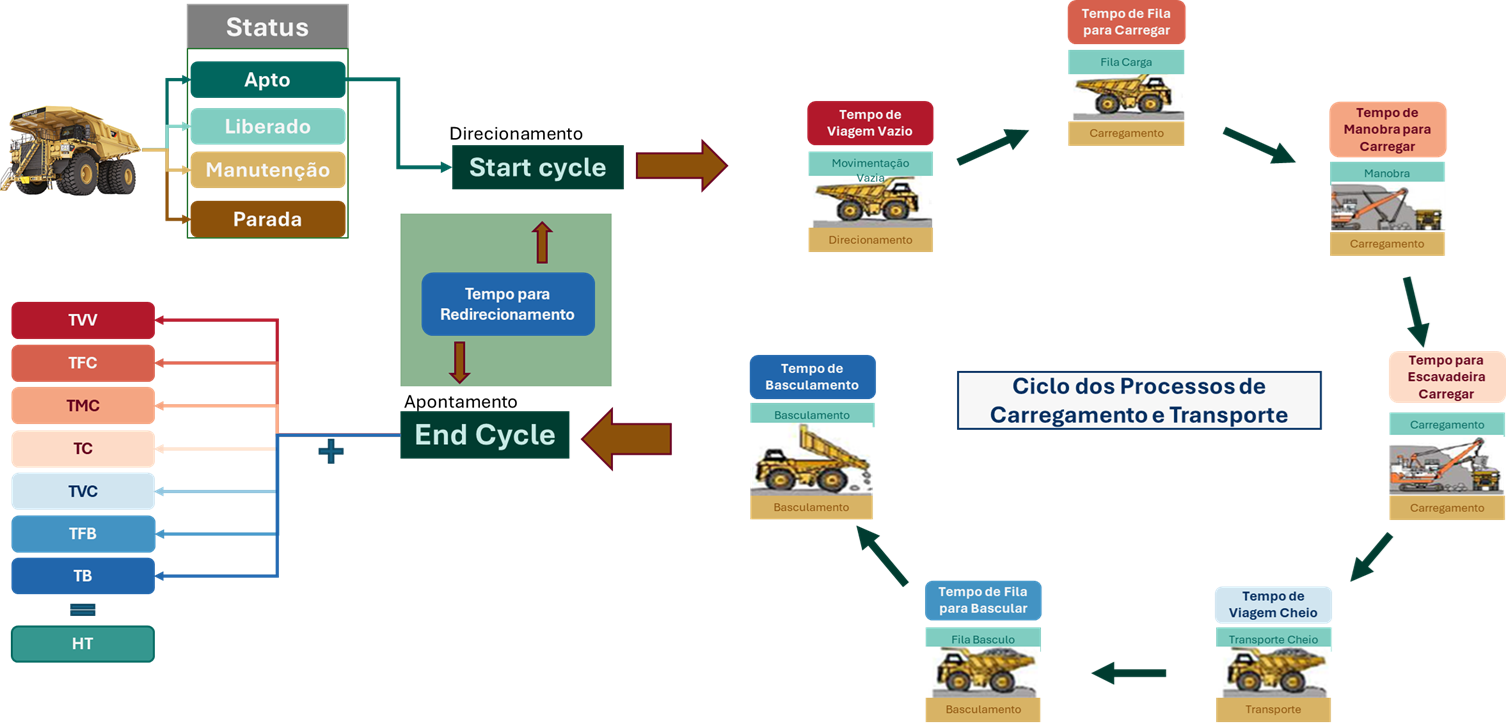
\includegraphics[keepaspectratio]{chapters/../images/fig-ciclo-processos.png}}

}

\caption{Ciclo de processos de carregamento e transporte.}

\end{figure}%

tempo de carregamento). Com o caminhão cheio, ocorre o transporte (TVC
-- tempo de viagem cheio), aguarda na fila para basculamento (TFB --
tempo de fila para bascular) e, finalmente, o basculamento (TB-- tempo
de basculamento). Para um único turno de trabalho da operação, um
determinado número de ciclos (NC) é realizado.

\begin{tcolorbox}[enhanced jigsaw, opacityback=0, leftrule=.75mm, colback=white, bottomrule=.15mm, colbacktitle=quarto-callout-note-color!10!white, rightrule=.15mm, colframe=quarto-callout-note-color-frame, coltitle=black, titlerule=0mm, opacitybacktitle=0.6, title=\textcolor{quarto-callout-note-color}{\faInfo}\hspace{0.5em}{Note}, toprule=.15mm, toptitle=1mm, arc=.35mm, left=2mm, bottomtitle=1mm, breakable]

O tempo total do ciclo influencia diretamente a produtividade da
operação e é afetado por fatores como distância de transporte, condições
da pista, eficiência do equipamento de carga e organização do tráfego.

\end{tcolorbox}

\section{Status do Equipamento}\label{sec-status-equipamento}

Como a medição é feita baseado em durações de tempo, os apontamentos são
realizados sempre que o caminhão alterar o seu status de operação,
estes, que são subdivididos em \textbf{4 classes}: apto para operação,
liberado pela manutenção, em manutenção ou em parada operacional.

Estas classes exercem um importante direcionamento das responsabilidades
de acompanhamento dos indicadores chaves de desempenho (ICDs) e possuem
problemas operacionais distintos. Por exemplo, quando o caminhão está:

\begin{itemize}
\item
  \textbf{``apto para operação'':} equipe de operação responsável e
  focada no ciclo de carregamento e transporte. Principal desafio:
  seleção e dimensionamento dos equipamentos. Segundo Mohtasham et
  al.~(2021), relaciona-se à escolha adequada dos equipamentos para
  manuseio ideal de materiais, resultando em melhoria da produtividade.
\item
  \textbf{``liberado pela manutenção'':} momento imediatamente posterior
  à execução da manutenção; transição de responsabilidade da manutenção
  para operação. Um acordo de nível de serviço (ANS) deve ser
  pré-estabelecido para eficiência na transição.
\item
  \textbf{``em manutenção'':} responsabilidade da equipe de manutenção,
  envolvendo planejamento, inspeção, programação e confiabilidade.
\item
  \textbf{``parada operacional'':} grandes paradas planejadas e
  gerenciadas considerando contingências; embora pertença à operação, o
  planejamento é conduzido pela gerência considerando toda a cadeia
  produtiva.
\end{itemize}

\section{Descrição do equipamento}\label{descriuxe7uxe3o-do-equipamento}

\subsection{Equipamentos de
transporte}\label{equipamentos-de-transporte}

\begin{figure}

{\centering \pandocbounded{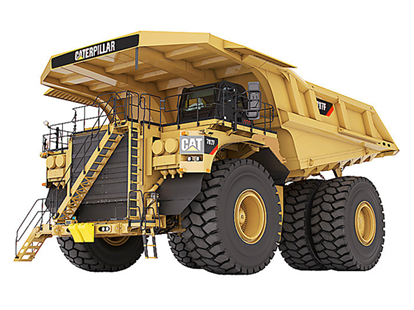
\includegraphics[keepaspectratio]{chapters/../images/fig-caminhao-797.png}}

}

\caption{Caminhão de mineração Caterpillar CAT® 797F. Fonte: Caterpillar
2022.}

\end{figure}%

Como mostrado na Figura @ref(fig:caminhao-797), o caminhão de mineração
Caterpillar CAT® 797F é objeto de estudo, impulsionado por motor de
combustível diesel, com capacidade de carga nominal útil (``payload'')
de 400 toneladas --- é um dos caminhões mais presentes nas frotas do
mercado brasileiro.

Logo, para identificar as principais causas que acarretam o baixo
desempenho dos indicadores de performance da manutenção dos caminhões
CAT® 797F, é preciso compreender os níveis de intervenção que são as
subdivisões de um sistema para os quais são realizadas as ações de
manutenção.

\subsection{Equipamentos de carga}\label{equipamentos-de-carga}

\subsection{Equipamentos de
infraestrutura}\label{equipamentos-de-infraestrutura}

\chapter{\ldots{} (restante do seu texto e código aqui)
\ldots{}}\label{restante-do-seu-texto-e-cuxf3digo-aqui}

\chapter{Análise de dados
recorrentes}\label{anuxe1lise-de-dados-recorrentes}

\section{Estrutura de banco de dados}\label{estrutura-de-banco-de-dados}

\subsection{Exemplos de histórico de
dados}\label{exemplos-de-histuxf3rico-de-dados}

\subsection{Tipos e classes dos dados}\label{tipos-e-classes-dos-dados}

\subsection{Categoria de horas}\label{categoria-de-horas}

Categoria de horas corresponde à divisão do tempo em classes de serviços
ou condição dos equipamentos, detalhando as horas na execução de
atividades de operação e manutenção no equipamento. Para melhor cálculo
dos indicadores, os tempos de funcionamento são agrupados em horas
dependendo da ocorrência dos eventos e do conjunto de equipamentos que
compõe o sistema.

No ciclo de processos de transporte, os dados coletados em caminhões
``off-highway'' são obtidos dos horímetros instalados no sistema de
medição e denominados tempos operacionais.

\begin{figure}

{\centering \pandocbounded{\includegraphics[keepaspectratio]{chapters/../images/fig-categorias-horas.png}}

}

\caption{Fluxo de relacionamento entre categorias de horas.}

\end{figure}%

A partir daí, estas são apontadas no banco de dados em categorias de
horas, que são as: horas efetivas (HEF), horas de atraso operacional
(HAO), horas trabalhadas diversas (HTD), horas trabalhadas de
infraestrutura (HTI); horas ociosas interna (HOI); horas ociosas externa
(HOE); horas de manutenção corretiva (HMC), horas de acidente (HAC);
horas preventivas sistemática (MPS) e horas preventivas não sistemática
(MPNS). Iremos denominar estes elementos com o tempo de primeiro nível.
Como mostrado na Figura @ref(fig-categorias-horas), o fluxo de
relacionamento entre estas categorias é ilustrado.

Para o cálculo de indicadores, é comum realizar a síntese de algumas
categorias de horas ou, de outra forma, a junção de horas. Assim, os
\textbf{elementos de tempo de segundo nível} são:

\begin{itemize}
\tightlist
\item
  \textbf{Horas de manutenção corretiva total} (HMCT = HMC + HAC)
\item
  \textbf{Horas de manutenção preventiva} (HMP = MPS)
\item
  \textbf{Horas trabalhadas não produtivas} (HNTP = HTI + HTD)
\item
  \textbf{Horas ociosas} (HO = HOI + HOE)
\item
  \textbf{Horas trabalhadas produtivas} (HTP = HEF + HAO)
\end{itemize}

Por fim, para o \textbf{terceiro nível} temos:

\begin{itemize}
\tightlist
\item
  \textbf{Horas trabalhadas} (HT = HEF + HAO + HTD + HTI)
\item
  \textbf{Horas em manutenção} (HM = HMC + HAC + MPS + MPNS)
\item
  \textbf{Horas ociosas} (HO)
\end{itemize}

Ao agrupar as categorias de horas em dia, semana, mês ou ano, o valor
nominal será dado pela soma da duração de todos os apontamentos, cuja
razão esteja configurada para contabilizar esta categoria. Em todos os
níveis a soma das categorias representam as \textbf{horas calendário}
(HC), por exemplo, temos que:

\[
HC = HT + HM + HO
\]

\begin{tcolorbox}[enhanced jigsaw, opacityback=0, leftrule=.75mm, colback=white, bottomrule=.15mm, colbacktitle=quarto-callout-note-color!10!white, rightrule=.15mm, colframe=quarto-callout-note-color-frame, coltitle=black, titlerule=0mm, opacitybacktitle=0.6, title=\textcolor{quarto-callout-note-color}{\faInfo}\hspace{0.5em}{Legenda das Categorias de Horas}, toprule=.15mm, toptitle=1mm, arc=.35mm, left=2mm, bottomtitle=1mm, breakable]

\begin{itemize}
\tightlist
\item
  \textbf{HMC}: Horas de Manutenção Corretiva
\item
  \textbf{HAC}: Horas de Aguardo Corretiva
\item
  \textbf{MPS}: Manutenção Preventiva Sistemática
\item
  \textbf{MPNS}: Manutenção Preventiva Não Sistemática
\item
  \textbf{HTI}: Horas de Trabalho Improdutivo
\item
  \textbf{HTD}: Horas de Trabalho em Deslocamento
\item
  \textbf{HOI}: Horas Ociosas Internas
\item
  \textbf{HOE}: Horas Ociosas Externas
\item
  \textbf{HEF}: Horas Efetivas
\item
  \textbf{HAO}: Horas de Apoio à Operação
\end{itemize}

\end{tcolorbox}

\subsection{Indicadores chave de desempenho
(ICD)}\label{indicadores-chave-de-desempenho-icd}

\subsection{Diagrama de build-up}\label{diagrama-de-build-up}

\section{Política de manutenção}\label{poluxedtica-de-manutenuxe7uxe3o}

\subsection{Manutenção corretiva}\label{manutenuxe7uxe3o-corretiva}

\subsection{Manutenção preventiva}\label{manutenuxe7uxe3o-preventiva}

\subsection{Dinâmica de ocorrência de
falhas}\label{dinuxe2mica-de-ocorruxeancia-de-falhas}

\subsection{Notações e
terminologia}\label{notauxe7uxf5es-e-terminologia}

\subsection{Gráfico de processo de
contagem}\label{gruxe1fico-de-processo-de-contagem}

\section{Confiabilidade e
periodicidade}\label{confiabilidade-e-periodicidade}

\subsection{Performance da
manutenção}\label{performance-da-manutenuxe7uxe3o}

\subsection{Mensuração de impacto na incidência de
corretivas}\label{mensurauxe7uxe3o-de-impacto-na-inciduxeancia-de-corretivas}

\subsection{Mensuração de impacto na
disponibilidade}\label{mensurauxe7uxe3o-de-impacto-na-disponibilidade}

\section{Indicadores Chave de Desempenho (ICD)}\label{sec-icd}

O principal produto do ciclo de transporte é a \textbf{massa
transportada (MT)}, este configura-se como elemento quantitativo.

Os ICDs são derivados de elementos de medição, logo, como um elemento
pode ser usado nas definições de vários ICDs, é improvável que eles
sejam independentes entre si. De acordo com @kang2016, há dois tipos
básicos de relacionamento, o primeiro dado pela relação de identidade
dos ICDs, baseado em suas definições e, o outro, é a relevância com
elementos de suporte compartilhados que podem ser obtidos por comparação
aos pares e/ou por agrupamentos em níveis.

Cada ICD revela um aspecto de desempenho para uma unidade de trabalho ou
sistema, derivado de dados monitorados de elementos de suporte. Os ICDs
podem ser agrupados por aqueles que representam um grupo de aspectos com
atributos semelhantes.

\subsection{Disponibilidade Física
(DF)}\label{disponibilidade-fuxedsica-df}

O ICD de \textbf{DF} indica a capacidade de um sistema estar em
condições de executar uma certa função, e sua indisponibilidade é devido
às horas de manutenção (HM), isto é, o indicador aponta para
oportunidades de melhoria relacionados à manutenção, e associados ao
status de ``em manutenção''.

\[
DF = \frac{HD}{HC} = \frac{HC - HM}{HC} \times 100\%
\]

Onde:

\begin{itemize}
\tightlist
\item
  \textbf{HD}: Horas Disponíveis
\item
  \textbf{HC}: Horas Calendário
\item
  \textbf{HM}: Horas de Manutenção
\end{itemize}

\subsection{Utilização Física (UF)}\label{utilizauxe7uxe3o-fuxedsica-uf}

De forma diferente, a \textbf{taxa de utilização física (UF)} leva em
consideração aspectos operacionais, sobre os quais a equipe de
manutenção não tem influência, ou seja, indica o quanto da
disponibilidade (HD) é utilizada efetivamente para operação (HT), logo,
o tempo não utilizado para operação corresponde à ociosidade do
equipamento (HO). Desta forma, temos que a ociosidade ocorre quando o
equipamento está em ``liberado pela manutenção'' ou ``parada
operacional''.

\[
UF = \frac{HT}{HD} \times 100\%
\]

\subsection{Produtividade (PR)}\label{produtividade-pr}

As horas trabalhadas (HT), são resultantes das ações de melhoria nos
demais indicadores e utilizadas para calcular tanto UF quanto o
indicador de \textbf{Produtividade (PR)}, este último, dado pelo
resultado da massa total transportada (MT) dividida por horas
trabalhadas (HT). Por conseguinte, a PR aponta para o ciclo dos
processos de carregamento e transporte, e está associado ao status
``apto para operação''.

\[
PR = \frac{MT}{HT}
\]

Onde \textbf{MT} é a massa total transportada (em toneladas).

\subsection{Perda de Produção por Indicadores}\label{sec-perda-producao}

Por fim, para o caso em que um sistema produtivo não cumpre as metas de
produção, é possível ainda calcular a \textbf{perda de produção por
indicadores de desempenho}, verificando a representatividade em
toneladas para cada indicador.

As equações de cálculo da perda de produção para cada indicador são
descritas a seguir:

\textbf{Perda de Produção por Disponibilidade Física:}

\begin{equation}\phantomsection\label{eq-perda-df}{
PP_{DF} = (HD_{programado} - HD_{realizado}) \times PR_{realizado}
}\end{equation}

\textbf{Perda de Produção por Utilização:}

\begin{equation}\phantomsection\label{eq-perda-uf}{
PP_{UF} = (HO_{realizado} - HO_{programado}) \times PR_{programado}
}\end{equation}

\textbf{Perda de Produção por Produtividade:}

\begin{equation}\phantomsection\label{eq-perda-pr}{
PP_{PR} = (PR_{programado} - PR_{realizado}) \times (HD_{programado} - HO_{realizado})
}\end{equation}

\begin{Shaded}
\begin{Highlighting}[]
\FunctionTok{library}\NormalTok{(dplyr)}
\FunctionTok{library}\NormalTok{(kableExtra)}

\CommentTok{\# Dados programados vs realizados}
\NormalTok{dados }\OtherTok{\textless{}{-}} \FunctionTok{data.frame}\NormalTok{(}
    \AttributeTok{Indicador =} \FunctionTok{c}\NormalTok{(}
        \StringTok{"Horas Calendário (HC)"}\NormalTok{, }\StringTok{"Horas Manutenção (HM)"}\NormalTok{,}
        \StringTok{"Horas Disponíveis (HD)"}\NormalTok{, }\StringTok{"Horas Ociosas (HO)"}\NormalTok{,}
        \StringTok{"Horas Trabalhadas (HT)"}\NormalTok{, }\StringTok{"Massa Transportada (MT)"}
\NormalTok{    ),}
    \AttributeTok{Programado =} \FunctionTok{c}\NormalTok{(}\DecValTok{720}\NormalTok{, }\DecValTok{72}\NormalTok{, }\DecValTok{648}\NormalTok{, }\DecValTok{65}\NormalTok{, }\DecValTok{583}\NormalTok{, }\DecValTok{140000}\NormalTok{),}
    \AttributeTok{Realizado =} \FunctionTok{c}\NormalTok{(}\DecValTok{720}\NormalTok{, }\DecValTok{95}\NormalTok{, }\DecValTok{625}\NormalTok{, }\DecValTok{88}\NormalTok{, }\DecValTok{537}\NormalTok{, }\DecValTok{125000}\NormalTok{),}
    \AttributeTok{Unidade =} \FunctionTok{c}\NormalTok{(}\StringTok{"h"}\NormalTok{, }\StringTok{"h"}\NormalTok{, }\StringTok{"h"}\NormalTok{, }\StringTok{"h"}\NormalTok{, }\StringTok{"h"}\NormalTok{, }\StringTok{"t"}\NormalTok{)}
\NormalTok{)}

\CommentTok{\# Calcular ICDs}
\NormalTok{icds }\OtherTok{\textless{}{-}} \FunctionTok{data.frame}\NormalTok{(}
    \AttributeTok{Indicador =} \FunctionTok{c}\NormalTok{(}
        \StringTok{"Disponibilidade Física (DF)"}\NormalTok{,}
        \StringTok{"Utilização Física (UF)"}\NormalTok{,}
        \StringTok{"Produtividade (PR)"}
\NormalTok{    ),}
    \AttributeTok{Programado =} \FunctionTok{c}\NormalTok{(}
        \FunctionTok{round}\NormalTok{((}\DecValTok{648} \SpecialCharTok{/} \DecValTok{720}\NormalTok{) }\SpecialCharTok{*} \DecValTok{100}\NormalTok{, }\DecValTok{1}\NormalTok{),}
        \FunctionTok{round}\NormalTok{((}\DecValTok{583} \SpecialCharTok{/} \DecValTok{648}\NormalTok{) }\SpecialCharTok{*} \DecValTok{100}\NormalTok{, }\DecValTok{1}\NormalTok{),}
        \FunctionTok{round}\NormalTok{(}\DecValTok{140000} \SpecialCharTok{/} \DecValTok{583}\NormalTok{, }\DecValTok{1}\NormalTok{)}
\NormalTok{    ),}
    \AttributeTok{Realizado =} \FunctionTok{c}\NormalTok{(}
        \FunctionTok{round}\NormalTok{((}\DecValTok{625} \SpecialCharTok{/} \DecValTok{720}\NormalTok{) }\SpecialCharTok{*} \DecValTok{100}\NormalTok{, }\DecValTok{1}\NormalTok{),}
        \FunctionTok{round}\NormalTok{((}\DecValTok{537} \SpecialCharTok{/} \DecValTok{625}\NormalTok{) }\SpecialCharTok{*} \DecValTok{100}\NormalTok{, }\DecValTok{1}\NormalTok{),}
        \FunctionTok{round}\NormalTok{(}\DecValTok{125000} \SpecialCharTok{/} \DecValTok{537}\NormalTok{, }\DecValTok{1}\NormalTok{)}
\NormalTok{    ),}
    \AttributeTok{Unidade =} \FunctionTok{c}\NormalTok{(}\StringTok{"\%"}\NormalTok{, }\StringTok{"\%"}\NormalTok{, }\StringTok{"t/h"}\NormalTok{)}
\NormalTok{)}

\CommentTok{\# Calcular perdas}
\NormalTok{PR\_real }\OtherTok{\textless{}{-}} \DecValTok{125000} \SpecialCharTok{/} \DecValTok{537}
\NormalTok{perdas }\OtherTok{\textless{}{-}} \FunctionTok{data.frame}\NormalTok{(}
    \AttributeTok{Tipo\_Perda =} \FunctionTok{c}\NormalTok{(}\StringTok{"Perda por DF"}\NormalTok{, }\StringTok{"Perda por UF"}\NormalTok{, }\StringTok{"Perda por PR"}\NormalTok{),}
    \AttributeTok{Calculo =} \FunctionTok{c}\NormalTok{(}
        \FunctionTok{paste0}\NormalTok{(}\StringTok{"("}\NormalTok{, }\DecValTok{648}\NormalTok{, }\StringTok{" {-} "}\NormalTok{, }\DecValTok{625}\NormalTok{, }\StringTok{") × "}\NormalTok{, }\FunctionTok{round}\NormalTok{(PR\_real, }\DecValTok{1}\NormalTok{)),}
        \FunctionTok{paste0}\NormalTok{(}\StringTok{"("}\NormalTok{, }\DecValTok{88}\NormalTok{, }\StringTok{" {-} "}\NormalTok{, }\DecValTok{65}\NormalTok{, }\StringTok{") × "}\NormalTok{, }\FunctionTok{round}\NormalTok{(PR\_real, }\DecValTok{1}\NormalTok{)),}
        \FunctionTok{paste0}\NormalTok{(}\StringTok{"("}\NormalTok{, }\FunctionTok{round}\NormalTok{(}\DecValTok{140000} \SpecialCharTok{/} \DecValTok{583}\NormalTok{, }\DecValTok{1}\NormalTok{), }\StringTok{" {-} "}\NormalTok{, }\FunctionTok{round}\NormalTok{(PR\_real, }\DecValTok{1}\NormalTok{), }\StringTok{") × "}\NormalTok{, }\DecValTok{583}\NormalTok{)}
\NormalTok{    ),}
    \AttributeTok{Perda\_ton =} \FunctionTok{c}\NormalTok{(}
        \FunctionTok{round}\NormalTok{((}\DecValTok{648} \SpecialCharTok{{-}} \DecValTok{625}\NormalTok{) }\SpecialCharTok{*}\NormalTok{ PR\_real, }\DecValTok{0}\NormalTok{),}
        \FunctionTok{round}\NormalTok{((}\DecValTok{88} \SpecialCharTok{{-}} \DecValTok{65}\NormalTok{) }\SpecialCharTok{*}\NormalTok{ PR\_real, }\DecValTok{0}\NormalTok{),}
        \FunctionTok{round}\NormalTok{((}\DecValTok{140000} \SpecialCharTok{/} \DecValTok{583} \SpecialCharTok{{-}}\NormalTok{ PR\_real) }\SpecialCharTok{*} \DecValTok{583}\NormalTok{, }\DecValTok{0}\NormalTok{)}
\NormalTok{    )}
\NormalTok{)}

\CommentTok{\# Apresentar resultados}
\FunctionTok{kable}\NormalTok{(dados, }\AttributeTok{caption =} \StringTok{"Dados Programados vs Realizados"}\NormalTok{) }\SpecialCharTok{\%\textgreater{}\%}
    \FunctionTok{kable\_styling}\NormalTok{(}\AttributeTok{bootstrap\_options =} \FunctionTok{c}\NormalTok{(}\StringTok{"striped"}\NormalTok{, }\StringTok{"hover"}\NormalTok{), }\AttributeTok{full\_width =} \ConstantTok{FALSE}\NormalTok{)}
\end{Highlighting}
\end{Shaded}

\begin{longtable}[t]{lrrl}
\caption{Dados Programados vs Realizados}\\
\toprule
Indicador & Programado & Realizado & Unidade\\
\midrule
Horas Calendário (HC) & 720 & 720 & h\\
Horas Manutenção (HM) & 72 & 95 & h\\
Horas Disponíveis (HD) & 648 & 625 & h\\
Horas Ociosas (HO) & 65 & 88 & h\\
Horas Trabalhadas (HT) & 583 & 537 & h\\
\addlinespace
Massa Transportada (MT) & 140000 & 125000 & t\\
\bottomrule
\end{longtable}

\begin{Shaded}
\begin{Highlighting}[]
\FunctionTok{kable}\NormalTok{(icds, }\AttributeTok{caption =} \StringTok{"Indicadores{-}Chave de Desempenho"}\NormalTok{) }\SpecialCharTok{\%\textgreater{}\%}
    \FunctionTok{kable\_styling}\NormalTok{(}\AttributeTok{bootstrap\_options =} \FunctionTok{c}\NormalTok{(}\StringTok{"striped"}\NormalTok{, }\StringTok{"hover"}\NormalTok{), }\AttributeTok{full\_width =} \ConstantTok{FALSE}\NormalTok{)}
\end{Highlighting}
\end{Shaded}

\begin{longtable}[t]{lrrl}
\caption{Indicadores-Chave de Desempenho}\\
\toprule
Indicador & Programado & Realizado & Unidade\\
\midrule
Disponibilidade Física (DF) & 90.0 & 86.8 & \%\\
Utilização Física (UF) & 90.0 & 85.9 & \%\\
Produtividade (PR) & 240.1 & 232.8 & t/h\\
\bottomrule
\end{longtable}

\begin{Shaded}
\begin{Highlighting}[]
\FunctionTok{kable}\NormalTok{(perdas,}
    \AttributeTok{caption =} \StringTok{"Análise de Perda de Produção"}\NormalTok{,}
    \AttributeTok{col.names =} \FunctionTok{c}\NormalTok{(}\StringTok{"Tipo de Perda"}\NormalTok{, }\StringTok{"Cálculo"}\NormalTok{, }\StringTok{"Perda (t)"}\NormalTok{)}
\NormalTok{) }\SpecialCharTok{\%\textgreater{}\%}
    \FunctionTok{kable\_styling}\NormalTok{(}\AttributeTok{bootstrap\_options =} \FunctionTok{c}\NormalTok{(}\StringTok{"striped"}\NormalTok{, }\StringTok{"hover"}\NormalTok{), }\AttributeTok{full\_width =} \ConstantTok{FALSE}\NormalTok{)}
\end{Highlighting}
\end{Shaded}

\begin{longtable}[t]{llr}
\caption{Análise de Perda de Produção}\\
\toprule
Tipo de Perda & Cálculo & Perda (t)\\
\midrule
Perda por DF & (648 - 625) × 232.8 & 5354\\
Perda por UF & (88 - 65) × 232.8 & 5354\\
Perda por PR & (240.1 - 232.8) × 583 & 4292\\
\bottomrule
\end{longtable}

Exemplo de cálculo de ICDs e perda de produção

\begin{tcolorbox}[enhanced jigsaw, opacityback=0, leftrule=.75mm, colback=white, bottomrule=.15mm, colbacktitle=quarto-callout-important-color!10!white, rightrule=.15mm, colframe=quarto-callout-important-color-frame, coltitle=black, titlerule=0mm, opacitybacktitle=0.6, title=\textcolor{quarto-callout-important-color}{\faExclamation}\hspace{0.5em}{Interpretação das Perdas}, toprule=.15mm, toptitle=1mm, arc=.35mm, left=2mm, bottomtitle=1mm, breakable]

A análise de perda de produção permite identificar qual indicador teve
maior impacto negativo na produção realizada, direcionando as ações de
melhoria:

\begin{itemize}
\tightlist
\item
  \textbf{Perda por DF}: Indica problemas de manutenção
\item
  \textbf{Perda por UF}: Indica problemas operacionais (ociosidade)
\item
  \textbf{Perda por PR}: Indica problemas de eficiência do ciclo
\end{itemize}

\end{tcolorbox}

\section{Resumo}\label{resumo}

🔔 \textbf{Pontos-chave:}

\begin{itemize}
\tightlist
\item
  O ciclo de carregamento e transporte é composto por etapas sequenciais
\item
  Status do equipamento define responsabilidades entre operação e
  manutenção
\item
  Elementos de suporte estruturam o cálculo dos ICDs através de
  categorias de horas
\item
  DF, UF e PR são os principais indicadores de desempenho
\item
  Perdas de produção podem ser mensuradas por indicador
\end{itemize}

\begin{center}\rule{0.5\linewidth}{0.5pt}\end{center}

\textbf{Próximo capítulo:} Fundamentos da Gestão da Manutenção

\chapter{}\label{section-1}

\chapter{}\label{section-2}

\chapter{}\label{section-3}

\bookmarksetup{startatroot}

\chapter{Summary}\label{summary}

In summary, this book has no content whatsoever.

\begin{Shaded}
\begin{Highlighting}[]
\DecValTok{1} \SpecialCharTok{+} \DecValTok{1}
\end{Highlighting}
\end{Shaded}

\begin{verbatim}
[1] 2
\end{verbatim}

\bookmarksetup{startatroot}

\chapter*{Referências}\label{referuxeancias}
\addcontentsline{toc}{chapter}{Referências}

\markboth{Referências}{Referências}

\phantomsection\label{refs}
\begin{CSLReferences}{0}{1}
\end{CSLReferences}

\section*{Recursos Adicionais}\label{recursos-adicionais}
\addcontentsline{toc}{section}{Recursos Adicionais}

\markright{Recursos Adicionais}

\begin{itemize}
\tightlist
\item
  \href{https://quarto.org/}{Documentação Quarto}
\item
  \href{https://r4ds.hadley.nz/}{R for Data Science}
\item
  \href{https://shiny.posit.co/}{Shiny Documentation}
\item
  \href{https://supabase.com/docs}{Supabase Documentation}
\end{itemize}


\backmatter


\end{document}
